\documentclass{scrartcl}% siehe <http://www.komascript.de>
\usepackage{selinput}% Eingabecodierung automatisch ermitteln …
\usepackage{hyperref}
\SelectInputMappings{% … siehe <http://ctan.org/pkg/selinput>
  adieresis={ä},
  germandbls={ß},
}
\usepackage{graphicx}
\usepackage[ngerman]{babel}% Das Beispieldokument ist in Deutsch,
                % daher wird mit Hilfe des babel-Pakets
                % über Option ngerman auf deutsche Begriffe
                % und gleichzeitig Trennmuster nach den
                % aktuellen Rechtschreiberegeln umgeschaltet.
                % Alternativen und weitere Sprachen sind
                % verfügbar (siehe <http://ctan.org/pkg/babel>).

\setlength{\parskip}{0.2cm}  % 2mm Abstand zwischen zwei Absätzen
\setlength{\parindent}{0mm}  % Absätze nicht einziehen
\usepackage[backend=biber,
isbn=false,                     % ISBN nicht anzeigen, gleiches geht mit nahezu allen anderen Feldern
sortlocale=de_DE,               % Sortierung der Einträge für Deutsch
%sortlocale=en_US,              % Sortierung der Einträge für Englisch
autocite=inline,                % regelt Aussehen für \autocite (inline=\parancite)
hyperref=true,                  % Hyperlinks für Ziate
style=ieee                     % Zitate als Zahlen [1]
%style=alphabetic               % Zitate als Kürzel und Jahr [Ein05]
%style=authoryear                % Zitate Author und Jahr [Einstein (1905)]
]{biblatex}
\addbibresource{literatur.bib}
\setlength{\bibitemsep}{1em}     % Abstand zwischen den Literaturangaben
\setlength{\bibhang}{2em}        % Einzug nach jeweils erster Zeile

% Trennung von URLs im Literaturverzeichnis (große Werte [> 10000] verhindern die Trennung)
\defcounter{biburlnumpenalty}{10} % Strafe für Trennung in URL nach Zahl
\defcounter{biburlucpenalty}{500}  % Strafe für Trennung in URL nach Großbuchstaben
\defcounter{biburllcpenalty}{500}  % Strafe für Trennung in URL nach Kleinbuchstaben

\begin{document}
% ----------------------------------------------------------------------------
% Titel (erst nach \begin{document}, damit babel bereits voll aktiv ist:
\titlehead{AMR}% optional
\subject{Projektbericht AMR}% optional
\title{Kartierung der WLAN Signalstärke}% obligatorisch
%\subtitle{Untertitel}% optional
\author{Florian Zirker, Lukas Arnecke}% obligatorisch
%\date{z.\,B. der Abgabetermin}% sinnvoll
\publishers{Prof. Dr. Thomas Ihme}% optional
\maketitle% verwendet die zuvor gemachte Angaben zur Gestaltung eines Titels
% ----------------------------------------------------------------------------
% Inhaltsverzeichnis:
\tableofcontents
% ----------------------------------------------------------------------------
% Gliederung und Text:

\section{Einleitung}
Eine moderne Hochschule ist auf eine funktionierende Netzwerkinfrastruktur angewiesen. Dazu gehört auch eine möglichst vollständige WLAN-Abdeckung, damit sowohl Studenten als auch Dozenten und Mitarbeiter ihre jeweiligen Aufgaben erfüllen können auch wenn sie sich nicht an einem fest installierten Rechner befinden.

Um genau diese WLAN-Abdeckung zu prüfen und eventuelle Lücken konkret aufzeigen zu können gab es im Rahmen der Vorlesung \textit{Autonome Mobile Roboter (AMR)} das Projekt, die Signalstärke mithilfe eines Roboters flächendeckend aufzeichnen zu können.

Zu diesem Zweck wurde auf einem Pioneer 3-DX die benötigte Hard- und Software installiert, um sowohl die eigene Position, als auch die Signalstärke des WLANs an diesem Punkt aufzuzeichnen.

Es ist uns gelungen, die Signalstärke des Eduroam Netzwerkes aufzuzeichnen und zu visualisieren. Die aufgezeichneten Werte zeigen, dass es möglicherweise sinnvoll wäre, zumindest in den Vorlesungsräumen ausreichend starke Router zu installieren, um dort die Verfügbarkeit von beispielsweise Vorlesungsunterlagen zu gewährleisten. Dieses Projekt ist aber mehr als Proof of Concept zu verstehen, weshalb es für eine genauere Aussage wichtig wäre, das gesamte Gebäude abzufahren, um eine flächendeckende Aussage treffen zu können.

\newpage
\section{Grundlagen}
\subsection{Pioneer 3-DX Roboter}
Der mobile Forschungsroboter Pioneer 3-DX ist eine Roboterplattform, die für fast alle Anwendungen modifizierbar ist. Er besteht im Grunde nur aus einem Motor, Reifen und einer Plattform, durch die benötigte Module angebracht werden können \cite{pioneer}. Die Steuerungseinheit ist so gebaut, dass sie über das \textit{Robot Operating System} (ROS) angesprochen werden kann.

\begin{figure}[h]
	\centering
	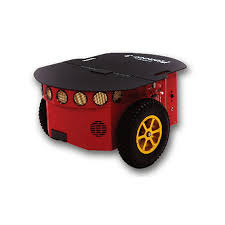
\includegraphics{bilder/pioneerRoh.jpg}
	\caption{Pioneer 3-DX Roboter ohne Aufbauten \cite{pioneer}}
	\label{pioneerRoh}
\end{figure}

Auf der Plattform ist ein Laser, ein Wlan-Modul und eine Rechner aufgebaut, mit deren Hilfe die Kartierung durchgeführt wird. Auf dem Rechner läuft Ubuntu 18.04 LTS, auf welchem wiederum ROS in der Version Melodic installiert ist.

\subsection{Robot Operating System}
\textit{ROS} ist ein Open Source Framework, welches speziell für auf die Nutzung für autonome Systeme entwickelt wurde. Die Idee von ROS ist die Bereitstellung von wiederverwendbaren Modulen, von denen jedes eine eigene Aufgabe erfüllen kann und die beliebig kombiniert werden können. Um die Module auch gut wiederverwenden zu können bietet ROS durch seine Paketverwaltung die Möglichkeit, von der Hardware zu abstrahieren. Es gibt dann ein Paket, welche für die Ansteuerung der Hardware zuständig ist und die dann über eine Steuerungseinheit wie ein Gamepad oder einen joystick angesteuert werden kann \cite{rosIntro}.

Für ein möglichst einfaches Management liefert ROS eine eigene Paketverwaltung, mit der die benötigten Pakete nachinstalliert werden können. Ein Paket enthält unter Anderem den Quellcode und Launchfiles für die \textit{Nodes}, in denen die Berechnungen stattfinden \cite{rosIntro2}. Jeder Node ist für andere Berechnungen zuständig, so gibt es einen Node für die Koordinatentransformationen zwischen den einzelnen Bauteilen des Roboters, einen für den Laserscanner, einen für die Berechnung der WLAN-Signalstärke und einen für die Ansteuerung des Motors.

Die Kommunikation zwischen Nodes, wie in  läuft über ein Publisher/Subscriber Prinzip, das bedeutet, dass ein Node, wie in Abbildung \ref{concept} dargestellt, definierte Informationen über einen \textit{Topic} veröffentlicht. Diese Topics können wiederum von anderen Nodes abgegriffen und weiter verarbeitet werden. Die enthaltenen Informationen werden über \textit{Messages} ausgetauscht, wodurch sowohl die Struktur als auch der Inhalt klar definiert sind. Alle Nodes müssen sich bei dem \textit{Master}, dem Namens- und Registrierungsservice innerhalb der ROS Umgebung, registrieren, um sich gegenseitig zu finden und dann auch Daten austauschen zu können \cite{rosKonzept}.

\begin{figure}
	\centering
	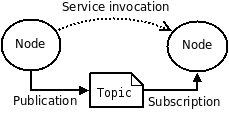
\includegraphics{bilder/ROS_concepts.png}
	\caption{Schematischer Aufbau der Kommunikation \cite{rosKonzept}}
	\label{concept}
\end{figure}

\subsection{Kartierung}
\label{kartierung}
Für die Kartierung bietet ROS das Package \textit{gmapping}, wenn die Karte mithilfe eines Lasermoduls erstellt werden soll. Dieses Package bietet die Funktionalität, um eine laserbasierte Karte mithilfe des Systems \textit{Simultaneous Localization and Mapping} (SLAM) zu erstellen. Hierbei wird eine 2D Karte aus der Kombination von den Laserdaten und der vermuteten eigenen Position erstellt. Die Daten über die eigene Position kommen aus den Odometriedaten, also der vermuteten Bewegungsrichtung und -distanz anhand der Bewegungen der Räder. Der Node \textit{slam\_gmapping} subscriped die Topics \textit{tf} und \textit{scan}, aus denen es dann die Karte berechnet und unter dem Topic map veröffentlicht \cite{gmap}. Die Abschätzung des Drehwinkels um die eigene Achse durch Odometrie ist vergleichsweise ungenau, weshalb es zu fehlerhaften Karten kommen kann, wenn der Roboter während der Kartierung zu viele Kurven fährt. Der Abgleich mit den Laserdaten wirkt diesem Effekt entgegen, bei einem erneuten Abfahren des Bereiches können entstandene Verschiebungen erkannt und behoben werden.


\subsection{Wireless Local Area Network}
\subsubsection{IEEE 801.11}
Der Begriff \textit{Wireless Local Area Network (WLAN)} beschreibt drahtlose Netzwerkkommunikation in einem Lokalen Netzwerk mit einer Übertragung über die Luft. Hierzu gehören viele Standards, zum Beispiel auch die Datennetze, die Bluetooth verwendet. In dieser Arbeit soll es aber um den Standard \textit{IEEE 802.11} gehen, ab hier unter dem Begrif "WLAN" referenziert wird. IEEE 801.11 spezifiziert neben der Übertragung per Radiowellen noch die Übertragung per Infrarot, um die es hier aber nicht gehen soll. IEEE 802.11 im Detail die Kommunikation in Funknetzwerken. Dies entspricht der Bitübertragungsschicht im ISO-OSI Modell. Der Standard besteht aus mehreren Unternormen, die nach und nach eingeführt worden sind. Die Wichtigsten sind:  802.11, 802.11a, 802.11b, 802.11g, 802.11n, 802.11ac, 802.11ad. Bei WLAN werden heute hauptsächlich zwei Frequenzbänder genutzt. Das 2,4 GHz und das 5GHz Band. Die Tabelle \ref{wlanStandards} zeigt die verschiedenen Generationen, deren Erscheinungsjahr und die Frequenz auf der sie senden und empfangen.

\begin{figure}[h]
	\centering
	\caption{Vergleich der WLAN Standards \cite{heiseWlan}}
	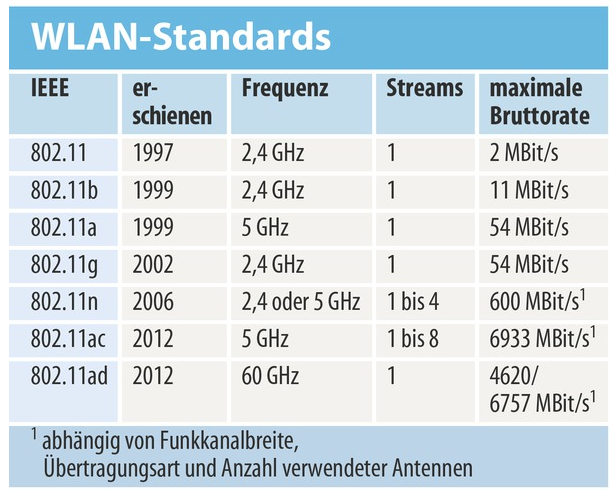
\includegraphics[width=10cm]{bilder/heise-de-wlan-standards}
	\newline
	\label{wlanStandards}
\end{figure}

Die verschiedenen Frequenzbänder haben unterschiedliche Eigenschaften. Im Vergleich hat das 2.4GHz eine höhere Reichweite. Ein Nachteil des 2.4GHz-Bandes ist, dass sich hier auch andere Funkstandards tummeln. Oftmals ist das 2.4GHz-Band durch viele Geräte sehr überfüllt. Im Gegenzug dazu ermöglicht das 5GHz-Band schnellere Übertragungsraten und bietet größere Kanalbandbreiten. Die Reichweite von WLAN kann bis zu 100m betragen, ist aber typischerweise auf einen oder wenige Räume begrenzt. 
Die Kommunikation zwischen zwei Teilnehmern in einem WLAN-Netz kann direkt im so genannten Ad-hoc-Modus oder im Infrastruktur-Modus mithilfe einer Basisstation auch Access-Point genannt erfolgen. Für uns hier relevant sind Verbindungen von mobilen Endgeräten zu Access-Points. Diese Basisstationen meistens mit den Routern des Netzwerkes verbunden. Somit kann eine Verbindung in das übergeordnete Netzwerk, zum Beispiel das Internet, erfolgen.

\subsubsection{SSID}
In der Hochschule Mannheim werden zum Bereitstellen eines flächendeckenden WLAN-Netzwerkes viele Basisstationen gleichzeitig eingesetzt. Um eine kontinuierliche Verbindung zu gewährleisten, auch bei sich bewegenden Mobilgeräten überlappen sich diese Bereich. 
Zusätzlich werden pro Basisstation mehrere Netzwerke bereitgestellt. Diese unterscheiden sich in dem Namen des Netzwerkes der so genannten \textit{Service Set Identifier (SSID)}. Dieser Eindeutige Name kann im Access-Point eingestellt werden. 

\subsubsection{Messen}

\begin{figure}[h]
	\centering
	\caption{Messen der Signalstärke mit der Android \textit{App Wifi Analyzer} (Die Netzwerknamen wurden unkenntlich gemacht)}
	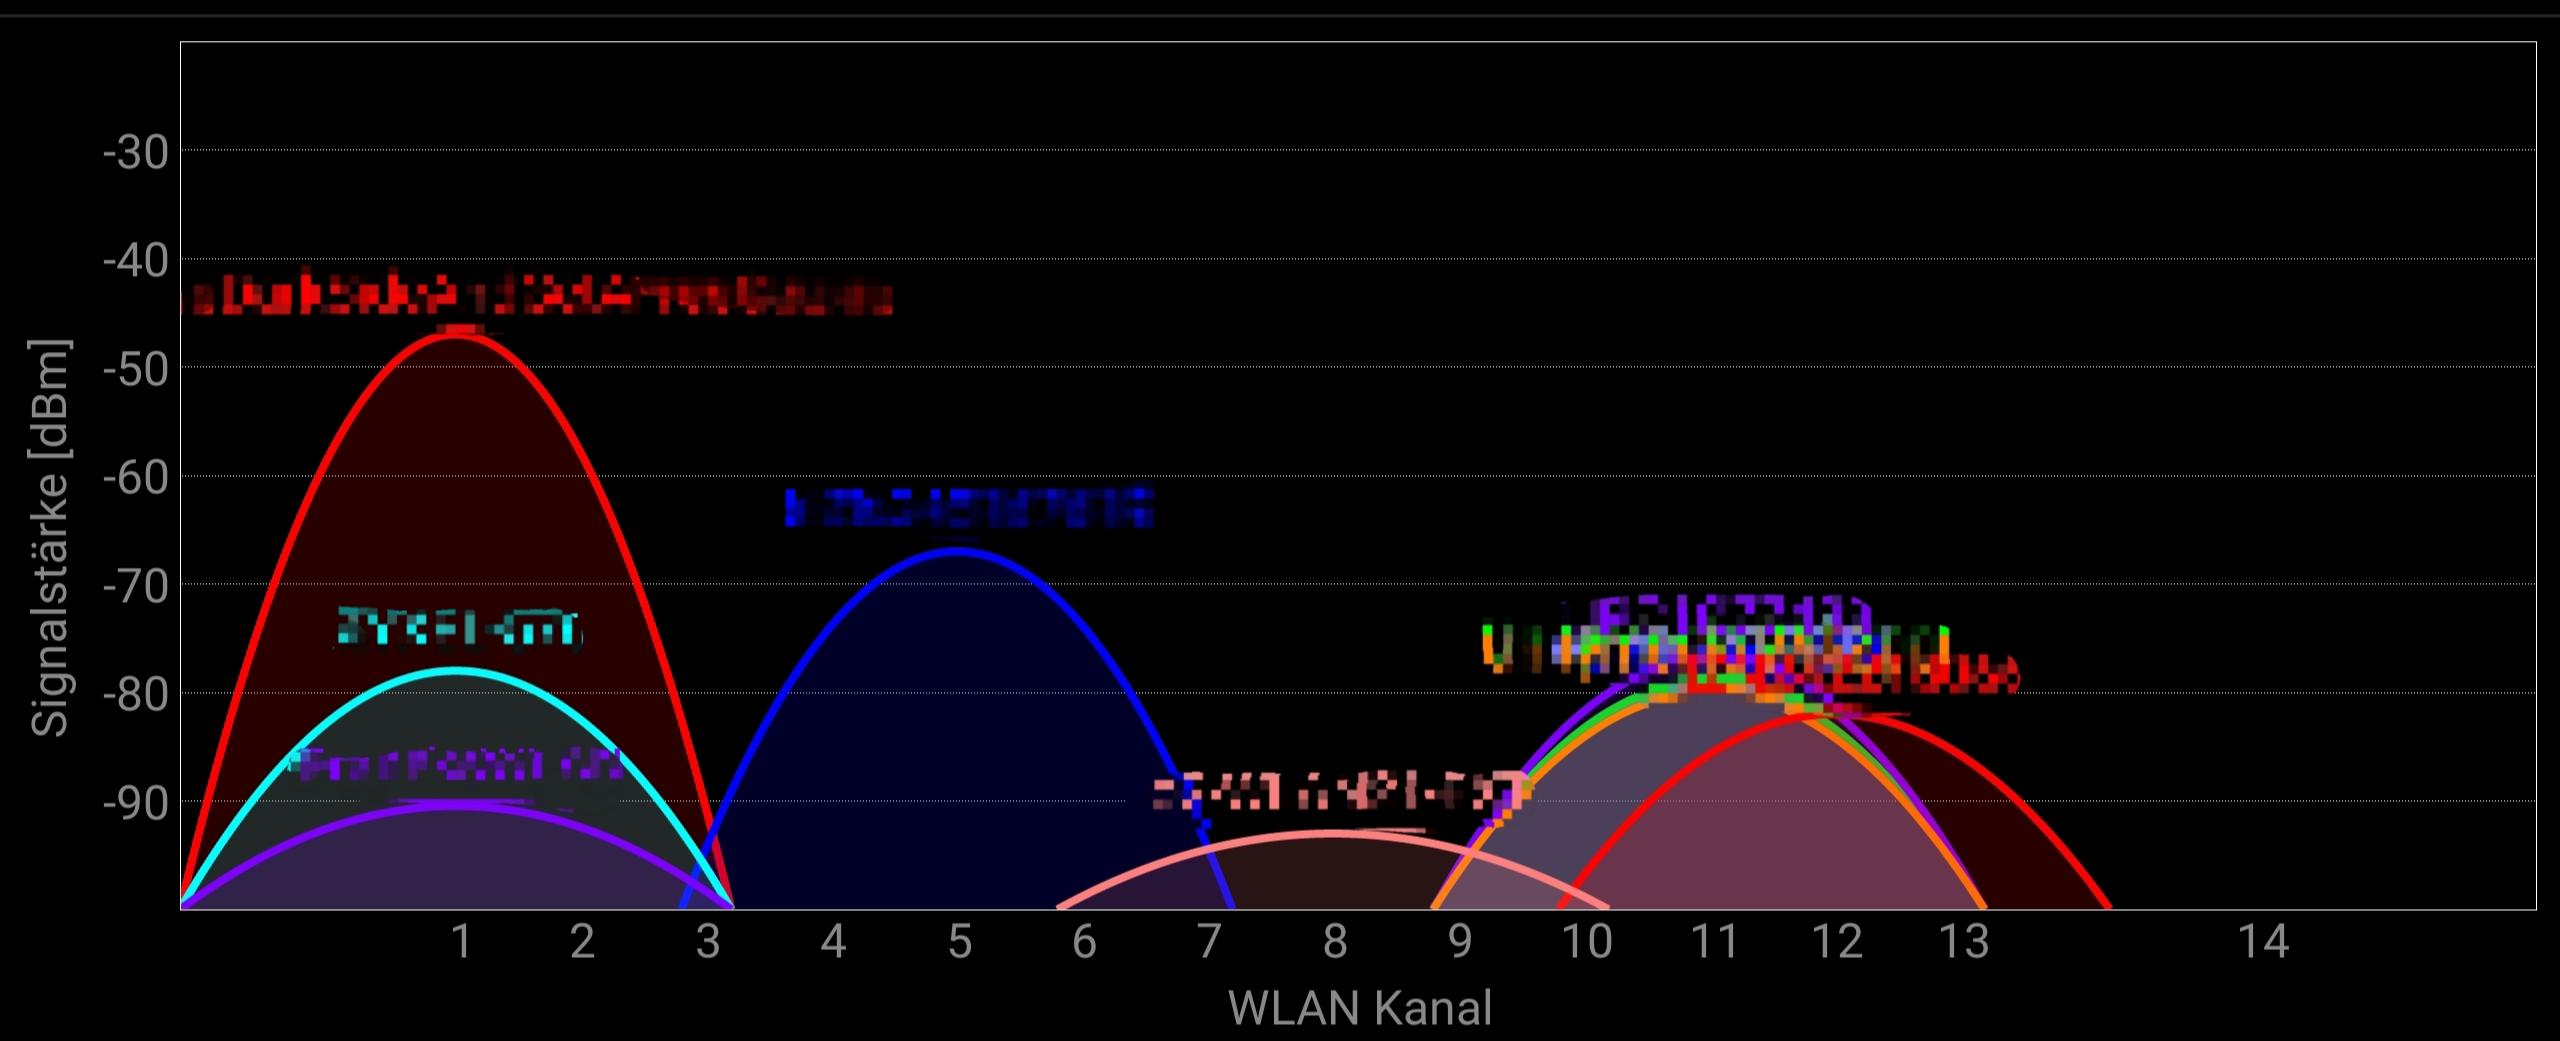
\includegraphics[width=10cm]{bilder/wifianalyzer}
	\newline
	\label{wifiAnalyzer}
\end{figure}

Um die Erreichbarkeit eines WLANs zu gewährleisten lohnt es sich die Signalstärke zu messen. Die Signalstärke ist Indikator für Stärke des ein kommenden WLAN-Signals an der WLAN-Schnittstelle. Somit kann man feststellen ob eine Signal stark genug ist um eine stabile Verbindung zu gewährleisten. Ein anderer Begriff dafür ist  \textit{Received Signal Strength Indication} oder auch RSSI-Wert. Gemessen wird sie in dBm, also die Dämpfung des signales. Je höher die Zahl, desto besser höher die Signalstärke. Unter Linux kann Signalstärke direkt  ausgelesen werden. Hierzu kann der Befehl "iwconfig" genutzt werden. Leider ist das Ergebnis stark von der verwendeten Hardware abhängig. Unter bestimmten Umständen wird nur ein Pseudowert ohne Einheit zurückgegeben.
Im Bild \ref{wifiAnalyzer} sieht man ein Screenshot einer Android Applikation mit der man die Signalstärke umliegender WLAN-Netzwerke messen und Anzeigen kann. Auf der X-Achse sind die verschiedenen Kanäle des 2,4GHz Bandes zu sehen. Die Y-Achse stellt die Signalstärke dar. Die ovalen, farbigen Ausschläge sind jeweils ein Netzwerk beschriftet mit der jeweiligen SSID.

Eine Andere Kenngröße ist die Verbindungsqualität, welche einer Pseudoeinstufung der Qualität der Verbindung entspricht. Diese wird aus mehreren Faktoren berechnet: Bitfehler, Übertragungsrate, Signalstärke, Synchronisationswerte und anderen Hardwaremetriken. Oftmals wird die Qualität als Bruch dargestellt. Beispiel: 41/70


Weitere Informationen über WLAN unter \cite{elektronikKompWlan}, \cite{elektronikKompWlanFreq}, \cite{heiseWlan}


\newpage
\section{Problemstellung}
% Eventuell können wir hier noch weiter unterscheiden: Inbetriebnahme, Kartierung und WLAN-Messung. Bin mir nicht sicher. FZ
Im Rahmen des Projektes gibt es verschiedene Problemstellungen, welche zwar aufeinander aufbauen, jedoch trotzdem in sich abgeschlossene Vorgaben beinhalten.

\subsection{Inbetriebnahme}
Der Stand des Roboters vor Beginn des Projektes war, dass auf dem aufgebautem Rechner Ubuntu 14.04 LTS installiert war, auf dem wiederum ein Dockersystem lief. ROS lief dann unter Docker, wodurch verschiedene Konfigurationen parallel auf einem Roboter genutzt werden konnten. Da die ROS Version sich mit der Ubuntuversion ändert lief hier entsprechend auch ROS Indigo.

Ziel ist es, auf eine neuere ROS Version umzusteigen, um auch neu implementierte Funktionen nutzen zu können. Daher muss neben ROS auch Ubuntu neu installiert und in diesem Zuge geprüft werden, ob an dem Ansatz mit Docker festgehalten wird.

\subsection{Kartierung}
Das neu installierte System soll eine Karte aus dem abgefahrenen Gebiet erstellen und diese anzeigen können. Hierbei sollte beachtet werden, dass die Karte sowohl durch manuelles Fahren erstellt werden kann, als auch eine bereits bestehende Karte hinterlegt werden kann, um dann nach dieser eine vorgegebene Strecke abzufahren. Im Hinblick auf das eigentliche Thema, das Kartieren der WLAN Signalstärke, liegt der Schwerpunkt jedoch entsprechend nicht auf der Umgebungskartierung.

\subsection{WLAN-Messung}
Neben der 2D Karte auf dem vorherigen Kapitel soll auch das WLAN kartografiert werden. Hierbei soll die Signalstärke für ein angegebenes Netz synchronisiert auf die aktuelle Position des Roboters aufgezeichnet werden.

Desweiteren soll eine Möglichkeit gefunden werden, die erhobenen Daten als Heatmap auf einer Karte zu visualisieren.

\newpage
\section{Realisierung}
\subsection{Genutzte Tools}
Für das Projekt wurde der Rechner auf dem Roboter komplett neu aufgesetzt. Für ein möglichst modernes System wurde Ubuntu 18.04 LTS installiert, wofür dann ROS in der Version Melodic vorgesehen ist und aus diesem Grund installiert wurde.

Als relevante Aufbauten auf dem Roboter ist als Laserscanner der \textit{Sick LMS-200} sowie als WLAN-Modul der \textit{EDIMAX EW-7811UAC} verbaut. Da der Roboter auch schon für andere Projekte benutzt wurde sind noch weitere Aufbauten bereits auf der Plattform verbaut, da sie aber für dieses Projekt nicht relevant sind wird hier nicht weiter darauf eingegangen.

Als bestehende ROS Pakete wurden genutzt:

\paragraph{gmapping}
Wie in Kapitel \ref{kartierung} bereits erwähnt dient das Paket \textit{gmapping} zur Erstellung einer 2D Karte aus einer Kombination von Informationen des Laserscanners und den Bewegungsdaten des Roboters. Diese Karte wird später als Grundlage verwendet, auf welcher dann die Heatmap erstellt wird.

\paragraph{p2os}
Das Paket \textit{p2os} enthält die Treiber und den Steuerungsnode für die Basis des für den Pioneer 3-DX. Er bildet die Schnittstelle zu der Hardware, wodurch wir uns damit nicht weiter auseinandersetzen müssen \cite{p2os}.

\paragraph{p2os\_teleop}
Um die Steuerung des Pioneer auch mit einem Gerät ansprechen zu können liefert das Paket \textit{p2os\_teleop} die Schnittstelle, um den Roboter auch mit einem Controller fahren zu können.


\subsection{Architektur}
%Löschen? Architektur ist im Grunde durch ROS vorgegeben und dazu gibt es keine Alternative. LA
Wir setzen auf ROS. Was wiederum auf dem Betriebsystem sitzt. Wir nutzen das Messaging-System (Publisher/Subscriber). Wir nutzen p2os was wiederum auf ??? nutzt. Wir schreiben unseren eigenen Knoten.

\subsection{Aufgetretene Probleme}
% Wollen wir  wirklich in einem Kapitel erklären was für Probleme wir hatten? Ich denke es macht mehr sinn die einzellnen Schritte genauer zu erklären und dann an der entsprechenden Stelle zu erklären was schwierig war. (Siehe folgende Kapitel)
ROS Melodic ist zwar veröffentlicht und für Ubuntu 18.04 vorgesehen, jedoch sind noch nicht alle Funktionen der Vorgängerversionen implementiert. Das führte dazu, dass manche Aufrufe der Launchscripte manuell umgeschrieben und ROS neu kompiliert werden musste.

Auch war das Extrahieren der Signalstärken erwies sich als Problem.
%Sollte Flo möglichst ausfüllen

\subsection{Inbetriebnahme und Installation}
% Alles veraltet. Vorhergehende Gruppe hat Docker ansazt gewält, nicht mehr lauffähig. Neues Betriebsystem. Neues ROS. Damit einige Probleme: Selbstcompilieren einiger Pakete nötig.
Wie bereits eingangs erwähnt wurde der Rechner des Roboters komplett neu gemacht. Damit das Betriebssystem möglichst lange laufen kann haben wir uns entschieden, Ubuntu 18.04 LTS zu installieren und darauf ROS Melodic aufzusetzen.

Während der Installation von ROS ist uns aufgefallen, dass diese Version noch nicht fertig implementiert ist. Der Code ist auf GitHub veröffentlicht, also konnten wir uns die Pakete herunterladen und manuell kompilieren. Hierbei sind dann Fehler aufgetaucht, dass einzelne Dateien nicht gefunden wurden. Nach einiger dieser Fehlermeldungen ist uns aufgefallen, dass ganze Unterordner von einem Ordner in einen anderen geschoben wurden und daher die Verweise innerhalb des Codes nicht mehr stimmen. Nach dem Anpassen der Dateien auf den neuen Pfad konnten die Pakete dann kompiliert werden.

\subsection{Simultaneous Localization and Mapping}
Als \textit{Simultaneous Localization and Mapping} (SLAM) bezeichnet das ermitteln der eigenen Position bei gleichzeitiger Erstellung der Karte. Daraus ergibt sich das Problem, dass eine Berechnung der eigenen Position ohne Kenntnis der Umgebung sehr schwer möglich ist. Ebenso ist ein Erstellen einer Karte ohne eigene Position ein Problem \cite{slam}. Das ROS Paket \textit{gmapping} nutzt SLAM, um genau dieses Problem zu lösen und eine recht genaue Karte zu erstellen. Dies hat auch bei den ersten Versuchen bereits funktioniert, als einziges Problem sollte man beachten, dass die erstellte Karte bei zu vielen Kurven verzogen ist, da sich durch ein jede Kurve der Einfluss der Odometrie vergrößert und diese fehleranfällig ist.

\subsection{Aufzeichnung der Fahrt}
Um die Karte auch nachträglich erstellen zu können haben wir uns dazu entschieden, die relevanten Messages aufzuzeichnen. Wir haben also eine Rosbag Datei erstellt, in der die Topics \textit{/tf}, \textit{/pose}, \textit{/base\_scan} und \textit{/wlan\_signal} gespeichert werden. Aus dieser Datei kann man auch nachträglich eine Karte erstellen und muss nicht für jeden Versuch bei der Auswertung der Daten neu mit dem Roboter fahren. Auch kann man so die Fahrt auch zuhause simulieren ohne Zugriff auf die Hardware. Der Topic /wlan\_signal ist selbst geschrieben und wir später noch genauer erklärt.

\subsection{Kartenerstellung aus aufgezeichneter Fahrt}
Die von gmapping bereitgestellten Informationen können in \textit{rviz} als Karte visualisert werden. Hierbei kann ausgewählt werden, welche Topics genau dargestellt werden sollen, da nicht alle laufenden Topics der Kartenerstellung dienen sondern auch beispielsweise Steuerungsfunktionen haben. Diese Karte wird dann im Kapitel \ref{nachverarbeitung} weiterverwendet, um die Signalstärken darzustellen.

\subsection{WLAN-Messung}
Um die WLAN Abdeckung zu messen sollte die Signalstärke ausgelesen und auf einem neuen Topic kontinuierlich veröffentlicht werden. Dafür wurde ein WLAN-USB-Stick gekauft und am Roboter eingerichtet. Auf der Kommandozeile in Linux kann man sich die Signalstärke mithilfe des iwconfig-Befehls sehr leicht ausgeben lassen. Es wurde über die Betriebsystemoberfläche eine Verbindung mit dem zu überwachenden WLAN-Netzwerk hergestellt. So konnte schnell ein Knoten geschrieben werden, der das Ergebnis des Linux Kommandos abfängt und auf dem Topic \textit{/wlanSignal} ausgibt. Hierfür wurde eine eigene Nachricht im ROS-Message-Format geschrieben.

Da die Frequenzbänder unterschiedliche Eigenschaften haben wurde entschieden, jeweils eine Messung für das 2,4GHz-Band und das 5GHz-Band zu machen und getrennt auszugeben um später differenzierte Ergebnisse zu erhalten. Die Idee war, zwei Netzwerkadapter anzusprechen und jeden über die Betriebssystemkonfiguration in ein separates Band zu hängen. Dies erwies sich aber als schwierig, da dies im WLAN-Standard so nicht vorgesehen ist. Für die neuen Modi, zum Beispiel IEEE 802.11n, müssen die WLAN-Karten auf beiden Bändern senden und empfangen können, da auch Dual-Chanel-Kommunikation möglich ist. Somit existiert keine Möglichkeit über das Betriebssystem ein Netzwerk-Interface ausschließlich auf ein Band zu konfigurieren. Außerdem war es problematisch, dass immer eine Verbindung zum Netzwerk vorhanden sein musste. Dies führte bei einem Wechsel der Basisstation, durch etwaiges Bewegen entlang der Flure, dazu, dass die kurzen Aussetzer der Messung in der Aufzeichnung sichtbar waren. 

Um die im Vorherigen Absatz genannten Probleme zu Lösen haben wir unsere Messung auf einen passiven Scanmodus umgestellt. Das bedeutet, dass man keine feste Verbindung mehr zu einem Netzwerk hat. Sondern \textit{alle} WLAN-Basisstationen in Reichweite mit deren Eigenschaften ausliest. Das können auch mehre pro Netzwerk sein. Da dies nicht mehr komfortabel über die Kommandozeile zu Realisieren ist, ohne Performanceverluste hin zunehmen, nutzten wir eine C++-Bibliothek Namens wifi-scan \cite{bmegliWifiScan}. Diese macht es möglich relativ einfach WLAN-Netzwerke auf einer bestimmten Netzwerkschnittstelle zu scannen. Nachdem diese noch geringfügig angepasst war, konnte eine Liste aller Access-Points in der Umgebung mit deren Eigenschaften (SSID, Signalstärke und Frequenz) ermittelt werden. Diese Liste konnte dann nach der gesuchten SSID gefiltert und sowohl die aktuelle als auch die maximale Signalstärke pro Band gefunden werden. Ein kleiner Nachteil dieser Lösung ist, dass der Knoten nun Administrationsrechte benötigt um den Scan durchzuführen. Dies wurde durch die Abfrage des Root-Passwortes beim Start des Knotens erledigt. 

% Hier kommt noch ein Bild rein wo man den rqt_graph für einen Scan sieht. 


\subsection{Nachverarbeitung}
\label{nachverarbeitung}
Es wurde ein Python-Skript geschrieben, welches die aufgezeichneten Rosbag-Dateien der Mess-Fahrten durchlief. Ziel war es eine CSV-Datei zu erhalten, die man im Nachgang plotten könnte. Das mit aufgezeichnete Topic /tf lieferte unter Zuhilfenahme der Transormation-API von ROS die transformierten genaue Position des Roboters. Die Transformation war nötig, da der Topic /pose nur die Position anhand der Odemetrie liefert, welche sehr ungenau ist. Die Transformations-Vektoren von /tf alleine sind auch nicht aussagekräftig, da sie nur die relative Verschiebung und der Drehwinkel liefern und nur durch kontinuierliches Integrieren und zusammen rechnen zu /pose die aktuelle Position liefern. Nachdem die CSV erstellt war konnte mit Matlab die Heatmap erzeugt werden.

Für die Visualisierung wurden zwei \textit{Scatterplots} aus der CSV erstellt, jeweils mit den Koordianten als Position und der jeweiligen Signalstärke des 2,4G und 5G Netzes zur Farbgebung. So entsteht ein 2D Koordinatensystem, bei dem an jedem Punkt der CSV ein Farbpunkt gesetzt ist, dessen Farbe dem Wert der Signalstärke entspricht. Hierbei wurde als Farbskala \textit{Jet} gewählt, welche in Abbildung \ref{skala} des folgenden Kapitels zu sehen ist. Anschließend war es möglich, die Schaubilder jeweils über die Karte zu legen und so die Position der Punkte in Abhängigkeit zu der Umgebung zu setzen.

\newpage
\section{Ergebnisse}
%Was ist raus gekommen. Neue Erkenntnisse, Lösungen, Unsere zwei Karten.
Der Pioneer-3dx Roboter konnte mit einer neuen Installation des Betriebssystems und neu Einrichtung des Robot-Operating-Systems neu in Betrieb genommen werden. Anschließend waren wir in der Lage  einen eigenen, neuen ROS-Knoten zu erstellen, der einiges an Funktionalität bietet. Hauptsächlich wird die Signalstärke eines bestimmten WLAN-Netzwerkes zuverlässig erfasst und auf einem ROS-Topic kontinuierlich veröffentlicht. Da diese Messung auf die zu verwende SSID und WLAN-Schnittstelle parametrisierbar ist, kann der WLAN-Scanner gut auf andere System portiert werden. Anpassungen und Erweiterungen der original p2os-Launchscripte führten dazu, dass die Kartierung mit nur einem Befehl gestartet werden konnte. Des weiteren konnten wir die Signale auf einer bei der Fahrt aufgezeichneten Karte visualisieren. 

% Das gehört hier nicht her --> Bitte nach Kartenerstellung verschieben (CSV-Teil in Nachverarbeitung teilw. schon enthalten)
%Zur Erstellung der Karten haben wir die Daten aus dem Map-Server von ROS exportiert und eine CSV Datei erstellt, bei der pro Zeitpunkt ein Eintrag geschrieben wird mit den aktuellen Koordinaten des Roboters und der dazugehörigen Signalstärken. Aus dieser Datei wurden dann in Matlab zwei Schaubilder erstellt, eines für die Signalstärke des 2,4G Netzes als Farbskala und eines für die 5G Signalstärke. Als Farbskala haben wir uns für die Jet Skala entschieden, die auch in Abbildung \ref{skala} dargestellt ist.

% Ab hier wieder Ergebnis
Als finales Ergebnis konnten zwei Schaubilder erstellt werden. Eines für die Signalstärke des 2,4G Netzes (Abbildung \ref{2g4}) und eines für die 5G-Signalstärke (Abbildung \ref{5g}). Diese zeigen die aufgezeichnete Fahrt des Roboters, die dabei erzeugte Karte und die Messungen der WLAN-Signalstärke im A-Gebäude der Hochschule Mannheim. Dabei entspricht die Farbgebung der Punkte der jeweiligen Signalstärke an dieser Position in der Karte. Wie in Abbildung \ref{skala} zu sehen ist, geht die Skala von Blau (-40dBm, gut) langsam über zu rot(-80dBm, schlecht).


\begin{figure}[h!]
	\centering
	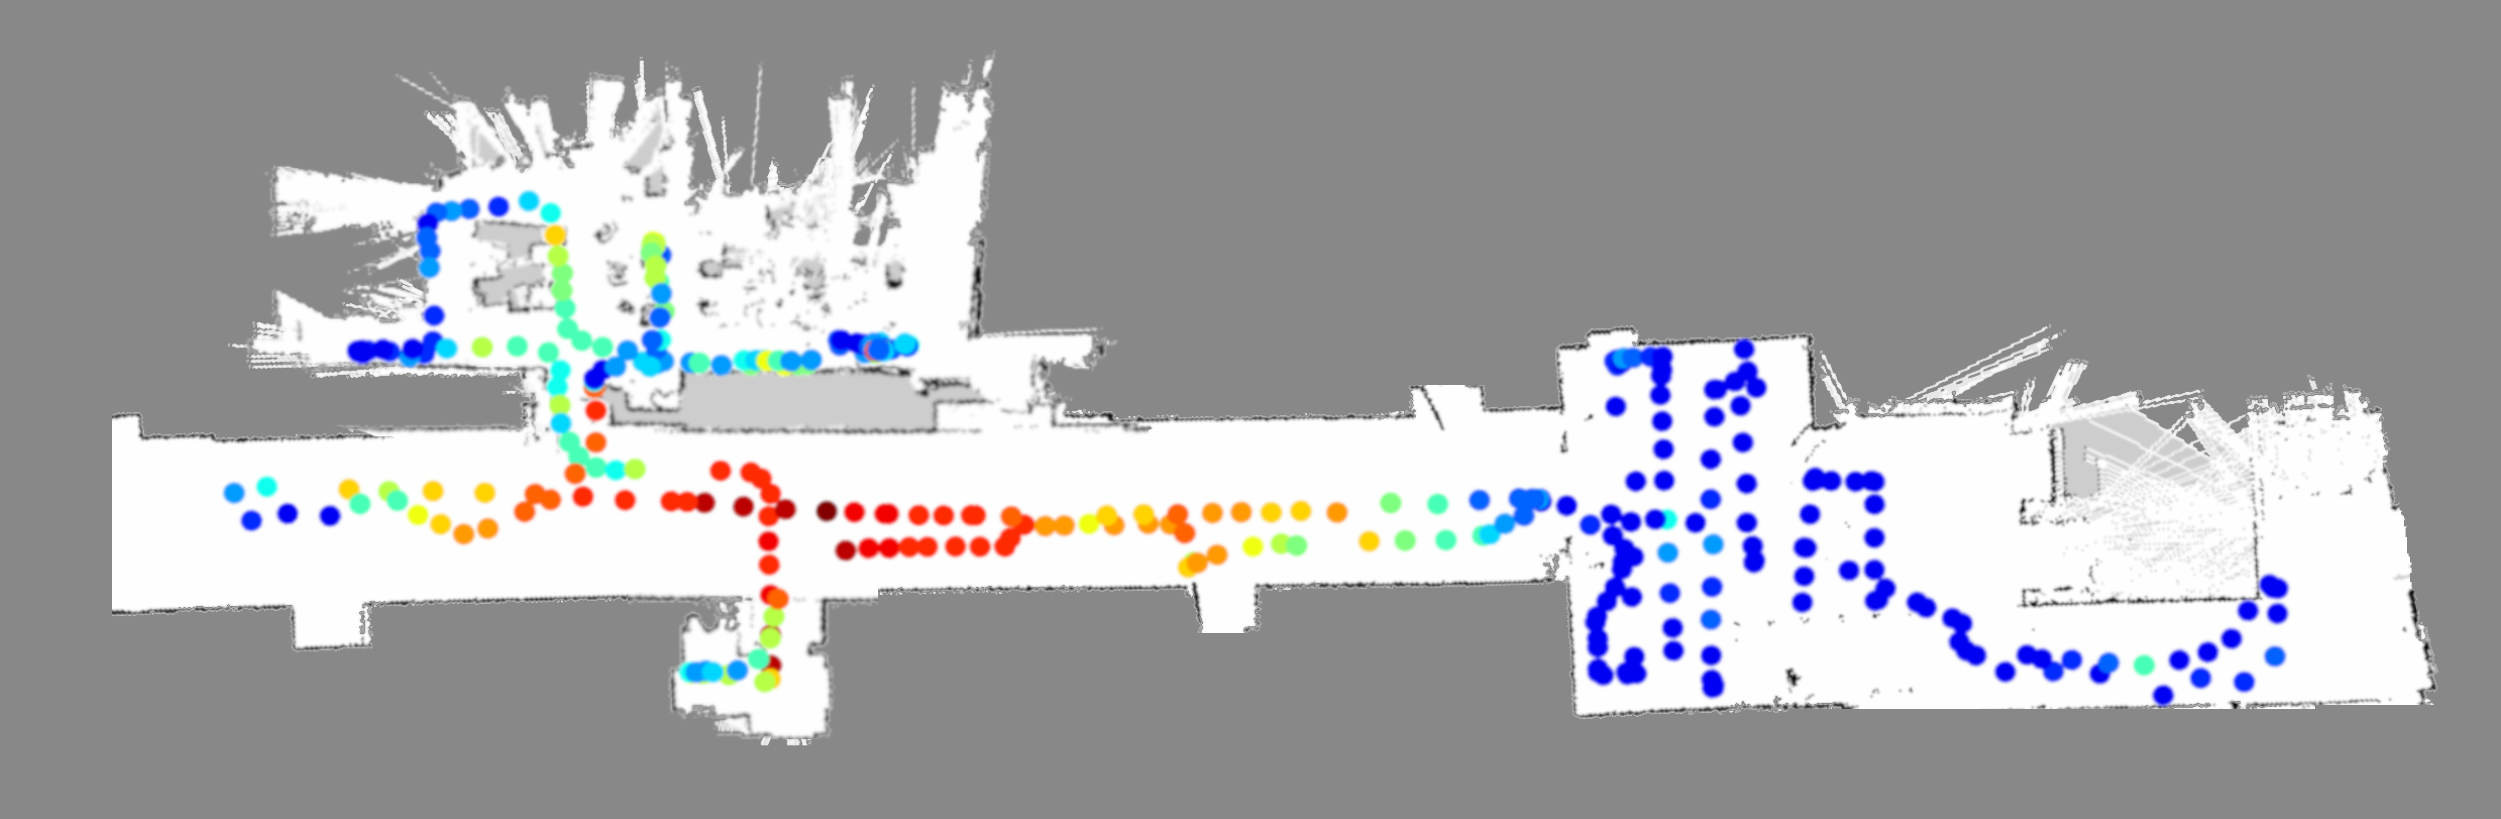
\includegraphics[width=\textwidth]{bilder/wlan-heatmap-2G4.png}
	\caption{Erstellte Karte aus der Signalstärke des 2,4G Netzes}
	\label{2g4}
\end{figure}

\begin{figure}[h!]
	\centering
	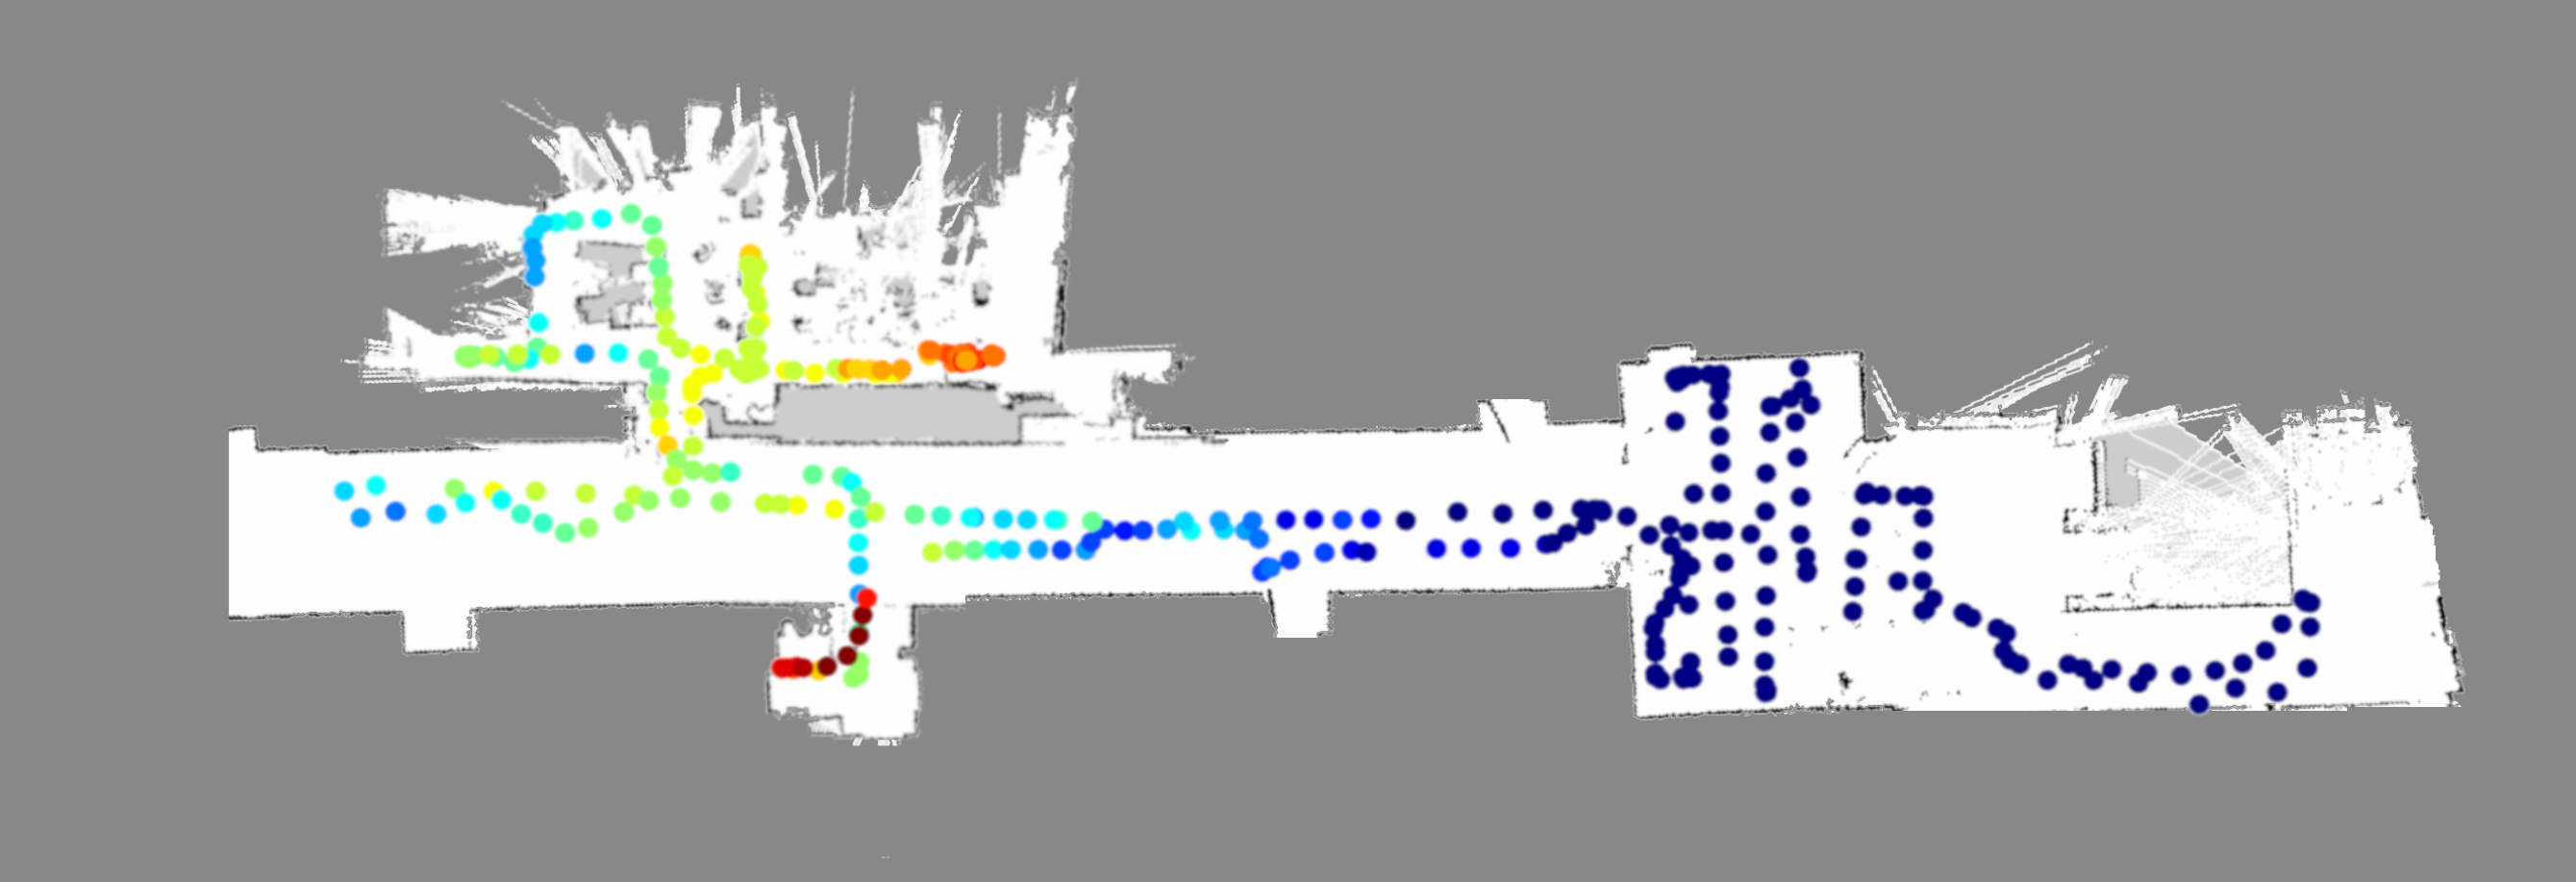
\includegraphics[width=\textwidth]{bilder/wlan-heatmap-5G.png}
	\caption{Erstellte Karte aus der Signalstärke des 5G Netzes}
	\label{5g}
\end{figure}

\begin{figure}[h!]
	\centering
	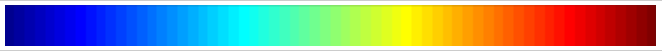
\includegraphics[width=\textwidth]{bilder/JetFarbskala.png}
	\caption{Jet Farbskala. Gutes Signal (links) zu schlechtem Signal (rechts)}
	\label{skala}
\end{figure}

%Warum ist dann mitten im Flur 5G besser? Sollte in der Signalstärke bei niedrigerer Reichweite und schlechterer Wanddurchdringung doch immer schlechter sein als 2,4G.
Als besonderer Punkt ist hier zu sehen, dass etwa in der Mitte des Flurs bei der Karte für das 2,4G Netz ein schlechtes Signal dargestellt wird, während es bei der 5G Karte vergleichsweise gut ist. Im Gegensatz dazu ist das Signal innerhalb des Robotik Labors oben links im Bild bei 2,4G besser ist als bei 5G. Als mögliche Erklärung kamen wir zu dem Schluss, dass 5G eine kleinere Reichweite hat und von Wänden schneller abgeschwächt wird. So ist es nachvollziehbar, dass der Roboter auf dem Flur ein stärkeres Signal zu einem entfernten Access-Point hat, jedoch in einem anderen Raum stärker abfällt, wenn das WLAN Signal durch eine Wand muss.

\subsubsection{Quellcode}
Alle programmierten Ergebnisse unseres Projektes können in unserem öffentlichen Repository auf Github.com eingesehen werden: \href{https://github.com/fzirker/wlan_pioneer}{Link zum wlan\_pioneer}

\newpage
\section{Ausblick}
Die Datenerhebung funktioniert, jedoch kann man gerade in der Nachbearbeitung noch einiges verbessern. So wäre ein Lösung, bei der die Heatmap direkt in rviz angezeigt und dann auch zusammen exportiert werden. Es gibt Ansätze für ein Paket, was genau das können soll, jedoch war dieses zum Zeitpunkt des Projektes nicht lauffähig, weshalb wir einen eigenen Node geschrieben haben.

Ein weiterer Punkt wäre ein Ansatz, mit dem der Roboter ein Gebiet strukturiert und selbstständig abfährt. So könnte man eine vorgefertigte Karte in Flächen einteilen und der Roboter muss in jeder Fläche mindestens einmal gewesen sein. So ist dann eine vollständige Abdeckung gewährleistet und es kann eine durchgängige Heatmap erstellt werden.

Ob es möglich ist, dass der Roboter selbstständig ein Gebiet kartografiert, anschließend diese Karte in Abschnitte unterteilt und abfährt könnte auch getestet werden. Da moderne Saugroboter dies teilweise machen wäre es durchaus vorstellbar.

\newpage
% Literaturverzeichnis erzeugen
\begin{flushleft}
	\printbibliography
\end{flushleft}


\end{document}
